\section{Methods}
\subsection{PCA for feature extraction}

PCA is an orthogonal transformation of data converting a vector $\mathbf{x}$ of
a high-dimensional feature space into a vector $\mathbf{y}$ of a lower
dimensional space. It does so by constructing an orthogonal subspace whose basis
define directions which capture most of the given data's variance. The elements
of the transformed vector $\mathbf{y}$ form the set of linearly uncorrelated
variables called \textit{principal compenents}. Mathematically the PCA can be
viewed as the statistical interpretation of the singular value decomposition
(SVD), in which the decomposed matrix $\mathbf{X}$ is the mean substracted or
centered data matrix.

Assuming the newly found basis is populated columnwise in a matrix $\mathbf{U}$,
the PCA performs a projection of vector $\mathbf{x}$ into vector $\mathbf{y}$,
which can be denoted by $\mathbf{y = UU^Tx}$. In PCA terminolgy, the columns of
$\mathbf{U}$ are called \textit{principal axis} while the already mentioned
\textit{principal components} are obatined by $\mathbf{U^Tx}$. The first
principal axis represents the largest variance of the data and is equal to the
eigenvectors belonging to the largest eigenvalue of the data's covariance
matrix. The following columns represent the next variances, all arranged in
decreasing order with respect to eigenvalues of the covariance matrix or the
singular values of centered $\MakeButtonField{X}$. Thus, the PCA components
arranged in the order according to their decreasing variance represent the most
important statistical information contained in the original set of data. 

\begin{figure}[ht]  
  \centering
  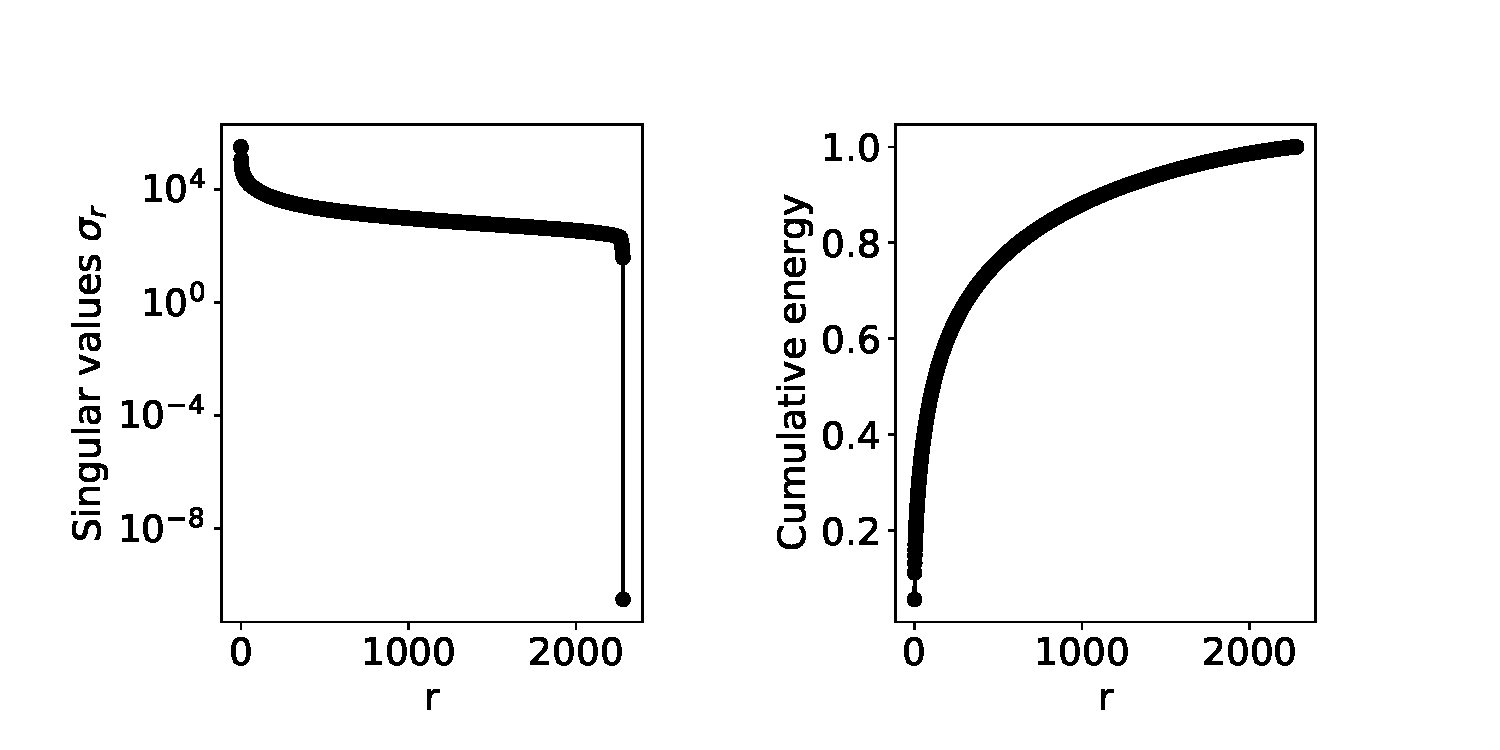
\includegraphics[width=\columnwidth]{singularValues.pdf}
  \caption{(left) Singular values $\sigma_k$ (right) Cumulative energy /
  variance captured by the first $r$ principal compenents in the Yale Face B
  Database}
  \label{sv}
\end{figure}

By limiting the number of principal components to the most important
eigenvalues, one achieves reduction of dimenstionality of data. As seen in Fig.
\ref{sv} it is possible to plot the singular values versus the number of
components. The amount of variance captured in the first $r$ modes can be
expressed by $\frac{\sum\limits_{k=1}^{r}{\sigma_k}}{\sum{\sigma_k}}$. This
gives a guideline on how many components to keep in order to capture a certain
amount of variance.

In Face recognition, the PCA or SVD decomposes the data into very intuitively
intrepretable components. Applied to a large library of facial images, the
principal axis are the so called \textit{eigenfaces}. They are the basis of the
newly computed coordinate system with which one can reconstruct old or even
generate completely new faces, meaning every face image in the original set of
data can be represented as a linear combination of these eigenfaces. Fig
\ref{eigenfaces} shows some of those eigenfaces. In appendix Fig.
\ref{appendix:reconstruction} I have included an example where I tried to
reconstruct a new face image with the eigenfaces of the Yale Face B Database
\cite{yalefaceB}. 

\begin{figure}[ht]
  \centering
  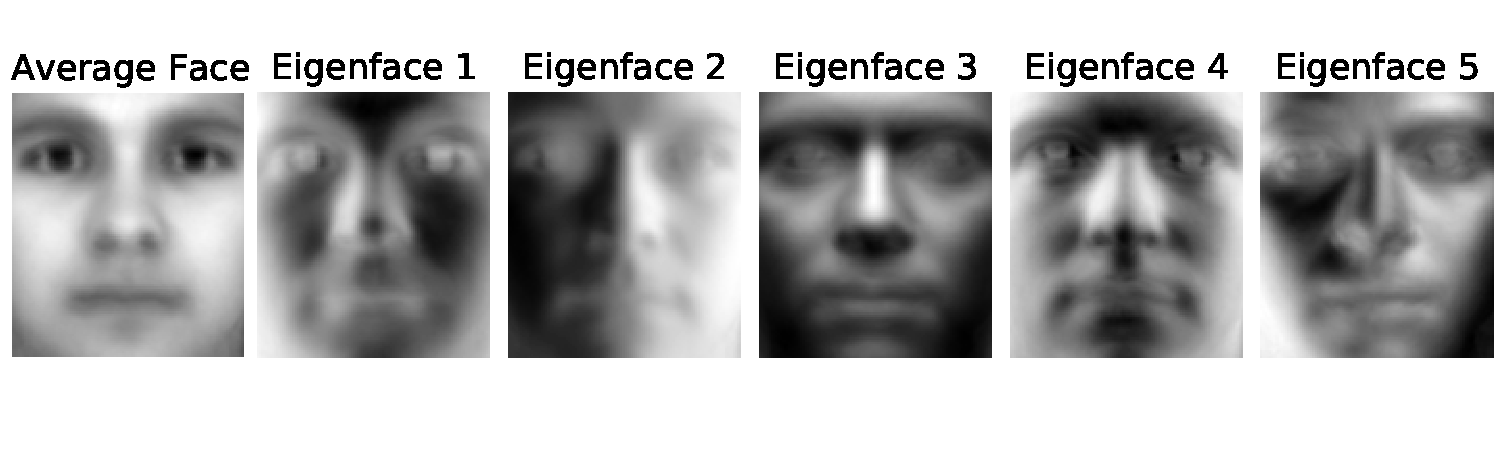
\includegraphics[width=\columnwidth]{eigenfaces.pdf}
  \caption{Average face and first five eigenfaces of the Yale Face Database B}
  \label{eigenfaces}
\end{figure}

Images of the same person tend to cluster in the eigenface space, making this a
useful tool for facial recognition and classification. A demonstration of PCA's
classification ability is shown in Fig. \ref{cluster}. For facial feature
extraction I will be using a chosen amount of principal components,
interpretable as the weights of the eigenfaces. These signals create the
patterns which are characteristic for the particular class/indviudal and
represent the coding of the image. They will serve as the input attributes to
the output classifier.

\begin{figure}[ht]
  \centering
  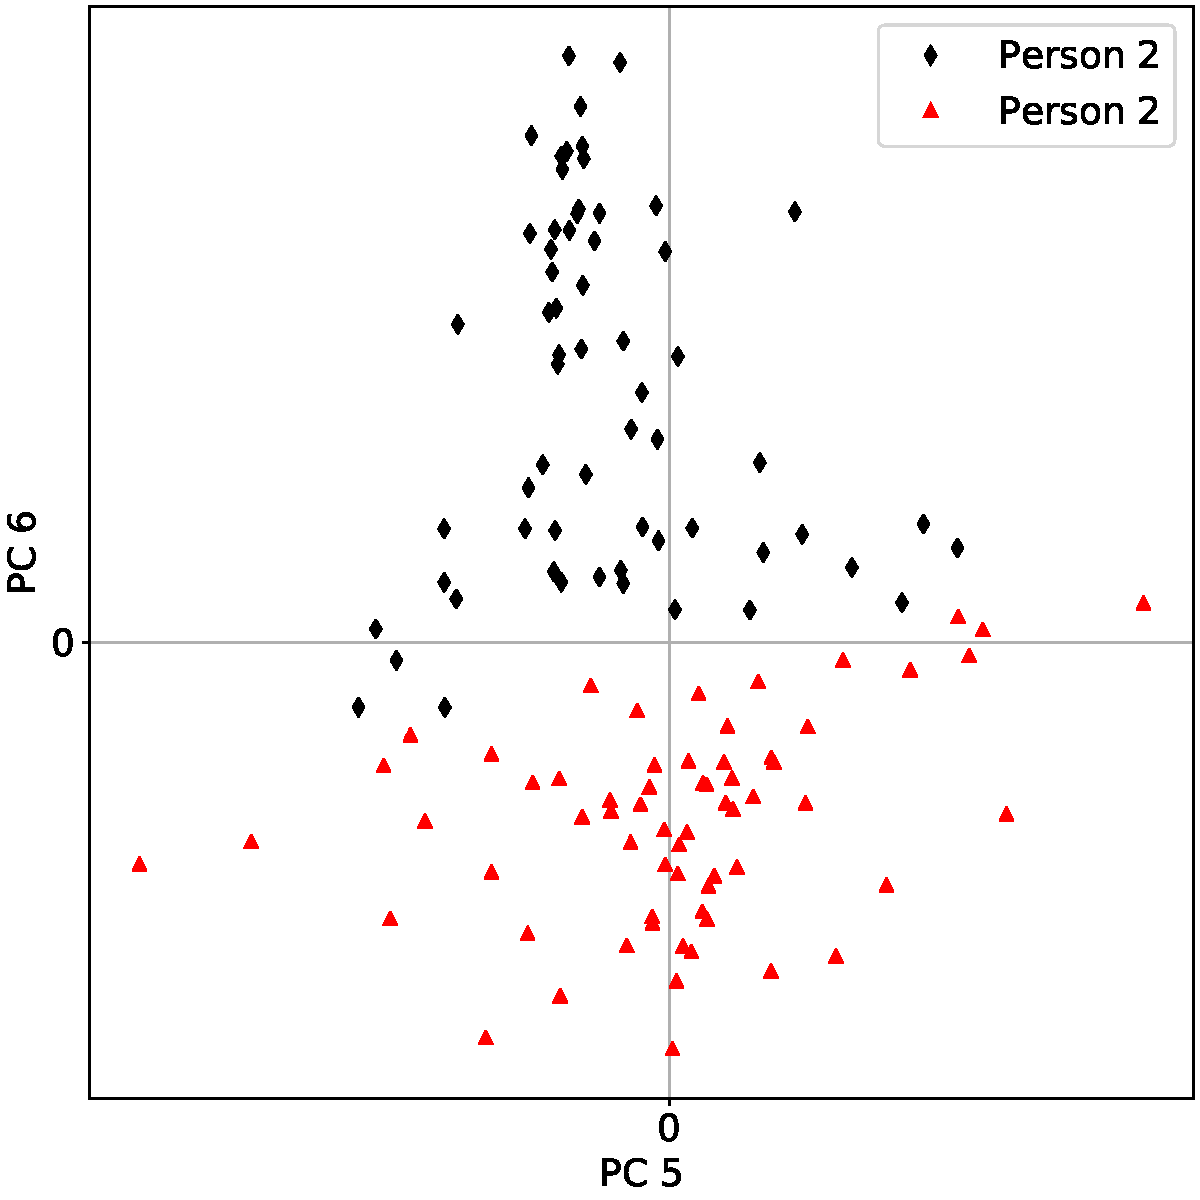
\includegraphics[width=0.7\columnwidth]{PCAcluster.pdf}
  \caption{Projection of all images from two individuals onto the 5th and 6th 
  PCA components}
  \label{cluster}
\end{figure}
